In the previous chapter was introduced the concept of Proof of Work, with a particular focus on the previous systems which gave inspiration to Satoshi Nakamoto's invention. In addiction, it was analyzed the problems that Proof-of-Work solves, such as double spending and consensus in an asynchronous distributed network.\\
The scope of this chapter is to dive more deeply into the Bitcoin mining theme, exploring how it actually works, the evolution in term of hardware used for the operations, and the differences between Solo Mining and Pooled Mining.\\

\noindent To better understand the basics of Bitcoin mining, since it's totally based on solving the above-described PoW (\ref{sec:pow}), a little reminder about hash functions is needed.
A \textbf{hash function} is a mathematical function that takes an input (of any size) and
produces a fixed-size string of characters, which is typically a sequence of alphanumeric characters. The output generated by a hash function is called "digest," or simply "hash". Hash functions are used in computer science and cryptography for many purposes, since the characteristic features of a hash function are:
\begin{itemize}
    \item Deterministic: for the same input, a hash function will always produce the same output. This property allows for consistent, verifiable and repeatable hashing.
    \item Fixed-size output: a hash function generates a hash value of a fixed length, regardless of the size of the input. For example, a hash function might always produce a 256-bit hash value.
    \item One-way (pre-image resistance): given a hash value, it is computationally infeasible to determine the original input. Basically, it should be extremely difficult to reverse-engineer the input given its hash value.
    \item Collision resistance: it should be highly improbable that two different inputs produce the same hash value. While collisions are theoretically possible a good hash function minimizes the chances of collisions.
\end{itemize}

\begin{figure}[h!]
\centering
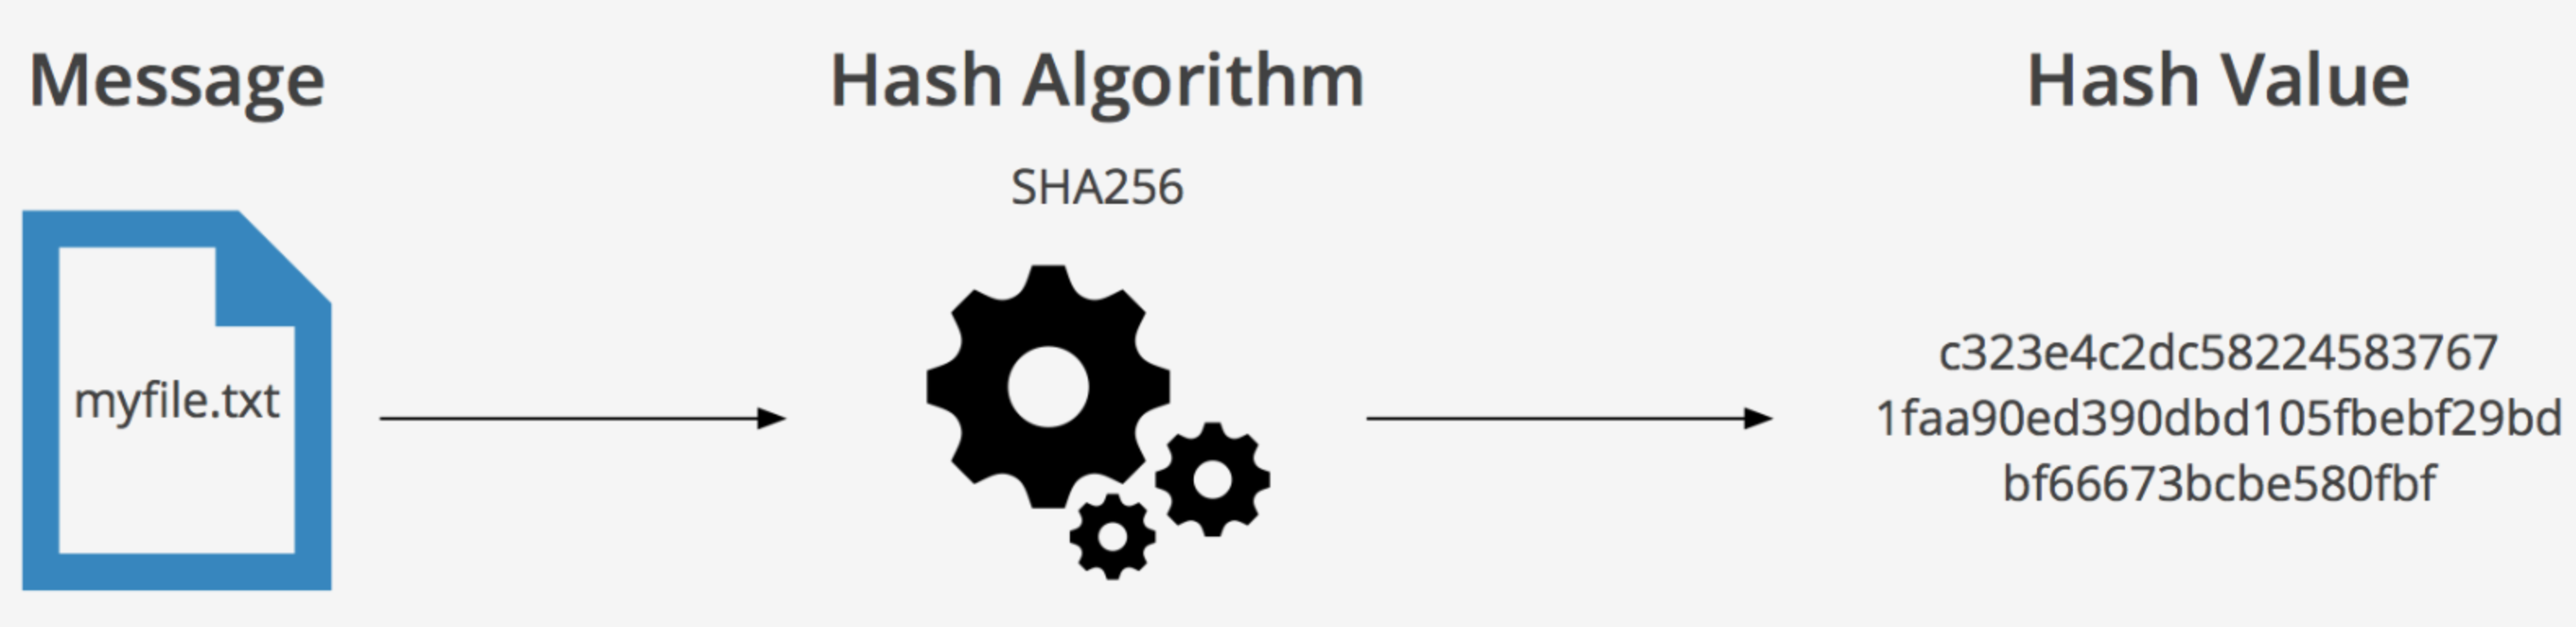
\includegraphics[width=15cm]{Figures/mining/sha256.png}
\caption{SHA-256 hash function in action}
\label{fig:sha256}
\end{figure}

\noindent In the case of Bitcoin, the hash function used is the SHA-256, as illustrated in Figure \ref{fig:sha256}.
